\textbf{Pregunta 8}
En algunas aplicaciones solo nos interesa el número de puntos que caen dentro de un rango
y no reportar cada uno de ellos. En este caso nos gustaría evitar el término $O(k)$ en el tiempo de consulta.

\begin{enumerate}
\item Describe cómo un árbol de rangos de una dimensión puede adaptarse para que una consulta así se pueda
  realizar en tiempo $O(\log n)$.
\item Usando la solución al problema para una dimensión, describe cómo se pueden responder consultas de
  conteo en rangos de $d$ dimensiones en tiempo $O(\log^d n)$.
\item Describe cómo se puede usar la técnica de cascada para mejorar el tiempo de consulta en un factor
  $O(\log n)$ para dos y más dimensiones.
\end{enumerate}


$\rhd$ \textbf{Solución:} A continuación se da solución a cada uno de los incisos:
\begin{enumerate}
\item[$a$)] La versión para una dimensión sería bastante simple, y de hecho sería
  como un árbol binario de búsqueda balanceado, pues basta con preservar el árbol
  general sin los árboles ``colgados'' que tiene el árbol de búsuqeda ortogonal.
  \newline
  
  La manera de ahorrar $\mathcal{O}(k)$ durante la búsqueda de rango, sería no recorrer las
  hojas del rango encontrado. Pues, basta con realizar dos recorridos hacia abajo desde la
  raíz, uno para encontrar la cota inferior del rango y otro para encontrar la cota superior.
  Así, y por la propiedad de tener mayores a la derecha y menores a la izquierda concluimos
  que las hojas entre las seleccionadas forman parte del rango.
\item[$b$)] De la misma manera, que en el caso de una dimensión, nos ahorramos $\mathcal{O}(k)$
  al no recorrer las hojas que quedan dentro del rango. Para generalizar a $d$ dimensiones basta
  reproducir la idea de los árboles ``colgados'', pues cada nodo que no sea hoja tendrá, inicialmente
  una referencia al árbol con coordenadas en $Y$. Luego los árboles con coordenadas en $Y$ tendrán
  colgados árboles con coordenadas en $Z$, y así de manera recursiva. Cuándo se requiera obtener
  el rango bastará con bajar por el árbol principal y recorrer cada árbol asociado de manera
  recursiva para inspeccionar que efectivamente el punto quede dentro del rango requerido.
  Cómo recorremos $\log n$ el árbol principal y por cada nodo distinto a una hoja recorremos
  su árbol asociado y a su vez los asociados recursivamente, entonces tenemos una complejidad
  de $k \cdot \log n$ dónde $k = \log m \cdot \log m' \dotsm \log m^{\dotsm} \approx \log^{d - 1} n$
  y concluimos que la complejidad en general por recorrido para encontrar un punto en el rango
  es de $\mathcal{O}(\log^d n)$.\newline
  
  Como esto se tiene que hacer para el punto ``menor'' en el rango y para el punto ``mayor''
  en el rango,  entonces tenemos una complejidad contenida en
  \[2 \cdot \mathcal{O}(\log^d n) \in \mathcal{O}(\log^d n).\]
\item[$c$)] Deseamos disminuir el número de operaciones en las consultas n-dimensionales. Basta dirigir
apuntadores a rangos menores, tal cómo se usan usualmente en una dimensión. A continuación un bosquejo
ilustrativo
\begin{center}
    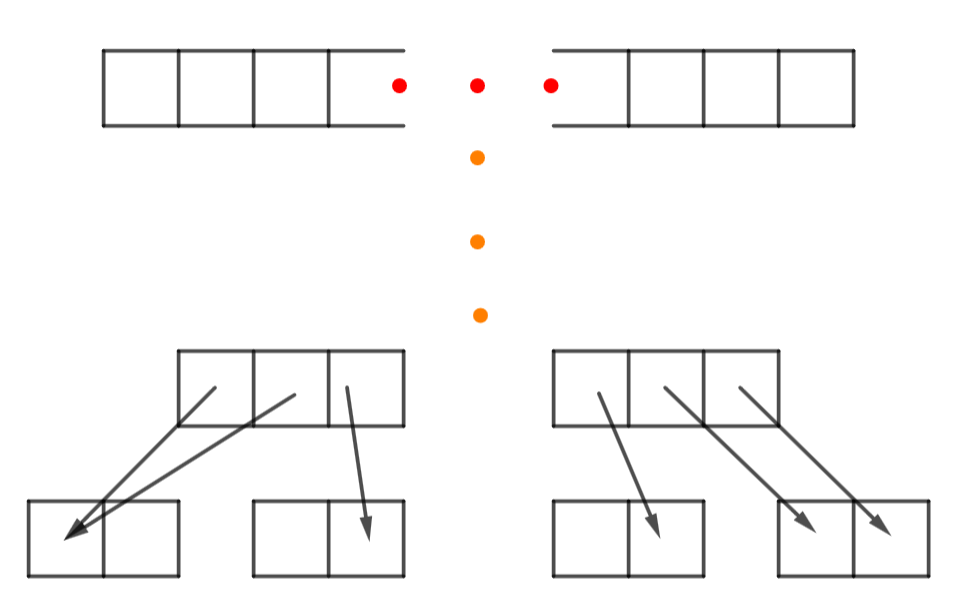
\includegraphics[scale=0.2]{Range1}
\end{center}
Sin embargo, lo anterior sólo nos funciona en una dimensión, ¿Cómo hacemos esto de manera n-dimensional?
Basta tener más apuntadores a una estructura similar que represente una segunda, tercera, ..., dimensión.
De esta manera sólo debemos descender en un árbol y buscar sus coordenadas en otros ejes sería sencillo
a través de redireccionamiento por medio de sus apuntadores. Esto es, por cada valor en el arreglo o subarreglo
debemos apuntar a su respectiva $y, z, \dotsm$ en estructuras similares. Cómo movernos por medio de estos
apuntadores es $\mathcal{O}(1)$, tenemos que la consulta se ve reducida a un orden $\mathcal{O}(\log_2 n)$.
\end{enumerate}
\hfill $\lhd$
